\documentclass{article}
\usepackage{tabularx,booktabs,ragged2e, graphicx}
%\newcolumntype{L}{>{\RaggedRight\arraybackslash}X}

\begin{document}
\oddsidemargin-1cm
\textwidth19cm
\begin{table}
\setlength\tabcolsep{6pt} % default value: 6pt
\centering
 \begin{tabularx}{\textwidth}{m{6cm} m{3cm} m{6cm} m{3cm}}
  
 \toprule
 Prediction & Pattern & Prediction & Pattern\\ [0.5ex]
 \midrule
 1. Total abundance (\textit{N}) should be lowest at low $\tau$ due to washout and at high $\tau$ due to low resource resupply.
 &
 \begin{minipage}{.3\textwidth}
 \includegraphics[width=20mm, height=20mm]{N-prediction}
 \end{minipage}
 &
 2. Productivity (\textit{P}) should be lowest at low $\tau$ due to washout and at high $\tau$ due to low resource resupply.
 &
 \begin{minipage}{.3\textwidth}
 \includegraphics[width=20mm, height=20mm]{ProdI-prediction}
 \end{minipage} \\
    
 \addlinespace
 3. Species richness (\textit{S}) should be lowest at low $\tau$ due to selection to resist washout and at high $\tau$ due to selection on persistence.
 &
 \begin{minipage}{.3\textwidth}
 \includegraphics[width=20mm, height=20mm]{S-prediction}
 \end{minipage}
 &
 4. Species evenness (\textit{E}) should be lowest at intermediate $\tau$, reflecting competition and the constraining influence of \textit{N} and \textit{S}.
 &
 \begin{minipage}{.3\textwidth}
 \includegraphics[width=20mm, height=20mm]{E-prediction}
 \end{minipage} \\
 
 \addlinespace
 5. Species turnover (\textit{W}) should decrease with $\tau$, reflecting less immigration and greater persistence. \textit{W} may then increase, due to loss of species at low \textit{S}.
 &
 \begin{minipage}{.3\textwidth}
 \includegraphics[width=20mm, height=20mm]{W-prediction}
 \end{minipage}
 &
 6. The percent of individuals in a dormant state should increase with greater $\tau$ due to insufficient resource resupply.
 &
 \begin{minipage}{.3\textwidth}
 \includegraphics[width=20mm, height=20mm]{Dorm-prediction}
 \end{minipage} \\
 
 \addlinespace
 7. Low $\tau$ should select for high intrinsic rates of growth. This selection pressure should decrease with increasing $\tau$.
 &
 \begin{minipage}{.3\textwidth}
 \includegraphics[width=20mm, height=20mm]{Growth-prediction}
 \end{minipage}
 &
 8. Low $\tau$ should select for high rates of active dispersal $\tau$. At high $\tau$, high rates of dispersal should be energetically wasteful. 
 &
 \begin{minipage}{.3\textwidth}
 \includegraphics[width=20mm, height=20mm]{Disp-prediction}
 \end{minipage} \\
 
 \addlinespace
 9. Increasing $\tau$ should select against high active basal metabolic rate (BMR) and select for greater the ability to grow  at a lower BMR.
 &
 \begin{minipage}{.3\textwidth}
 \includegraphics[width=20mm, height=20mm]{BMR-prediction}
 \end{minipage}
 &
 10. Resource specialization should decrease with $\tau$, where individuals are challenged to use any available resource.
 &
 \begin{minipage}{.3\textwidth}
 \includegraphics[width=20mm, height=20mm]{Spec-prediction}
 \end{minipage} \\
 
 \addlinespace
 11. Increasing $\tau$ should select for lower rates of resuscitation, as frequent resuscitation may be energetically wasteful.
 &
 \begin{minipage}{.3\textwidth}
 \includegraphics[width=20mm, height=20mm]{Resuscitation-prediction}
 \end{minipage}
 &
 12. Increasing $\tau$ should select for a greater reduction of basal metabolic rate (BMR) in dormancy.
 &
 \begin{minipage}{.3\textwidth}
 \includegraphics[width=20mm, height=20mm]{reducBMR-prediction}
 \end{minipage} \\
 
 \addlinespace
 13. The difference between active BMR and $1/\tau$ represents the match between resource supply and maintenance. \textit{N} should be greatest when BMR = $1/\tau$.
 &
 \begin{minipage}{.3\textwidth}
 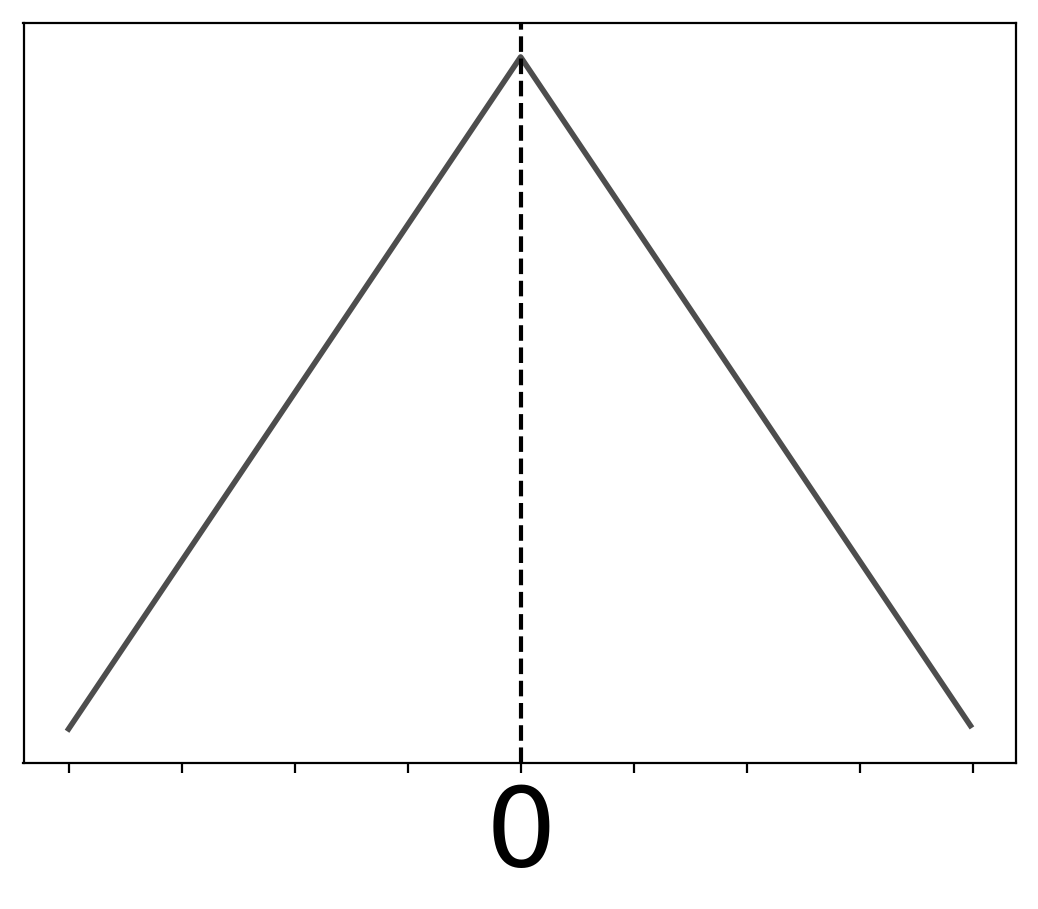
\includegraphics[width=20mm, height=20mm]{BMR-N}
 \end{minipage}
 &
 14. The difference between active BMR and $1/\tau$ represents the match between resource supply and maintenance. \textit{P} should be greatest when BMR = $1/\tau$.
 &
 \begin{minipage}{.3\textwidth}
 \includegraphics[width=20mm, height=20mm]{BMR-Prod}
 \end{minipage} \\
 
 \bottomrule
\end{tabularx}
\end{table}
\end{document}